\chapter{Introduction to Python}

\section{Introduction}

In this lab, we will learn the basic elements of the python
programming language: basic types, control flow, and functions.



\begin{plot}
\end{plot}
Use python complex type variables to compute $\sqrt{1+i}$.



\begin{itemize}
 \item dynamic variable assignment
 \item mutable vs immutable
\end{itemize}  




\section{Introduction}






Downloaded windows installer from:
  https://repo.anaconda.com/miniconda/Miniconda3-latest-Windows-x86\_64.exe

This log will also make it easier to get help if you have problems.

If you run into problems, do some research on Google to become
informed and to see if you can overcome the problem on your own
before asking for help.  This is an important technique in getting
help with technical problems that will serve you well in life.  You
will more easily get useful technical help, from the sort of people
most capable of offering it, when it is clear from your question that
you are informed and have already tried all of the obvious things.  If
you are still stuck after trying to solve the problem for yourself,
then contact your TA or instructor with specific technical details
about what is failing, and include your installation log.

If you find a problem with these instructions or manage to overcome a
technical problem yourself, make sure to note it in your log.

\section{Installing Miniconda3}

We will be using Miniconda3 based on Python 3.7 for data analysis
using Jupyter notebooks.  Miniconda is a lightweight package which we
can use to install all of the remaining analysis software we will need
in a consistent manner across all different operating systems.

Determine which OS type and version you have on the desktop or laptop
computer that you will be using for your coursework.  The software
here will work under Windows, Linux, or macOS.  You should also check
whether you have a 32-bit or 64-bit OS (you can find instructions for
how to determine this for your particular OS version with a Google
search.)  Most desktop or laptop computers built in the last ten years
are 64-bit.  If you are using Linux or macOS, then from within a
terminal type "echo \$SHELL" to determine the shell you are using
(typically "bash" these days).  Record all of this information in your
installation log file.

Once you have determined your OS type and version, follow the
instructions below approprate to your operating system.

\subsection{Installing under Windows}

If you have already installed a version of conda (e.g. Anaconda or
Miniconda) then you do not need to re-install it.  Instead, find the
the Anaconda Prompt in the Application menu and run it.

If you need to install Miniconda3, then download and run the
appropriate installer from:

%https://docs.conda.io/en/latest/miniconda.html\#

If prompted, you should choose to:

1) Accept the license / terms of use.
2) Install for just the current user, not all users.

Once installed, check that you can run the "Anaconda Prompt" and from
the prompt, you can run:

  conda --version

noting the output in your installation log.  Then proceed to
"Installing Physics 40 the Conda Environment".

\subsection{Installing Miniconda3 under Linux or macOS}
--------------------------------------------

If you believe you already already have a version of conda installed
(such as miniconda or ananconda) , check by running

   conda --version

If you see something like:

  conda 4.8.3

as output (even if the version is different) then you do have it
installed with the base environment activated, and can skip ahead to
the "Physics 116C Conda Environment” section.

If instead you get the message:

   conda: command not found

then either you have not installed any version of conda yet, or your
base environment is not initialized.  If you know how to initialize
your base environment, go ahead and do so, and then try the "conda
--version" test again.  If you do not know how to do so, it's probably
easiest to just proceed with these instruction, but you could read
ahead to the discussion on initializing the base environment and see
if you can get it working.

To install Miniconda, download the appropriate installer for your OS
here:

  https://docs.conda.io/en/latest/miniconda.html\#

For macOS, you can choose between a "package" or "bash" version. I
find it easier to follow the bash version, but the package version
will work too. I recommend you make the following choices described
below.  

1) Accept the license / terms of use.

2) Do not install for all users, but just one the current user.

3) You might be asked whether or not to allow the installer to issue
"conda init".  Answering "yes" will set some environment variables
persistently in your shell (i.e. they'll be set every time you log in
unless you do something to change them.)  This is convenient, but
there's a small chance that it might interfere with other software
which you have setup on your laptop, or just annoy you by advertising
"base" at every command prompt for the rest of your life.  If you are
concerned about such things, you should answer "no" when asked about
allowing the installation program to issue "conda init".  The downside
is that you'll have to explicitly activate the conda environment each
time you wish to use it, which is described below.  This is what I do,
because I use tools like Xilinx petalinux which is *very* fussy about
the user environment.

During the installation, take note of the following and record them in
your installation log:

1) The actual install location of miniconda.

2) Instructions for activating conda's base environment, if you choose
"no" to the "conda init" question.

After the installation, check for "conda --version" as described
above.  If the test works, your base environment is activated.  Record
the version number you are using in your installation log, and move on
to "Installing Physics 116C Conda Environment".

If you need to activate the base environment first, then there are
a few options.  If you noted instructions during installation, they
probably were something like:

  To activate conda's base environment in your current shell session:

  %eval "\$(/home/mulhearn/miniconda3/bin/conda shell.YOUR_SHELL_NAME hook)"

So in my case, I can start my anaconda environment with:

  %eval "\$(/home/mulhearn/miniconda3/bin/conda shell.bash hook)

because I use "bash" as my shell.  Another approach, which doesn't
seem to be officially supported but works fine for me, is to simply
source the appropriate startup script directly, e.g.:

  source ~/miniconda3/etc/profile.d/conda.sh

or:

  source ~/miniconda3/etc/profile.d/conda.csh

depending on your shell, and where you should replace ~/miniconda3/
with whatever directory contains your miniconda installation.

With your base environment activated, check for "conda --version" as
described above.  If the test works, record the version number you are
using in your installation log, and move on to "Installing Physics
116C Conda Environment".

\section{Installing the Physics 40 Conda Environment}

Start your conda base environment.

Make sure your conda is fully up to date with:

  conda update conda

then follow the prompts, e.g. selecting "y" as needed to update any out-of-date packages.

We'll be using a conda environment specifically for 116C to avoid
conflicts with any other projects on your computer, and to ensure that
we all have the same software installed.  To create our environment:

  conda create -n phy40 python=3.7 numpy scipy matplotlib ipython jupyter

\section{Starting the Physics 40 Conda Environment and Jupyter Notebook}

Start your conda as described above, then activate the 116 environment with:

  conda activate phy116

Then launch jupyter notebook with:

  jupyter notebook

When you are done with Phy 116 for the day you can deactivate the environment with:

  conda deactivate

\section{Starting a Jupyter notebook}

This course will make extensive use of the Jupyter Notebook interface
to Scientific Python, which is well suited to academic work (including
independent research) because it combines code with output in
digestable chunks.  Even when the end product is a polished peice of
software, much of the development occurs in the sort of interactive
sessions that Jupyter Notebooks provide.  

\begin{figure}[htbp]
\begin{center}
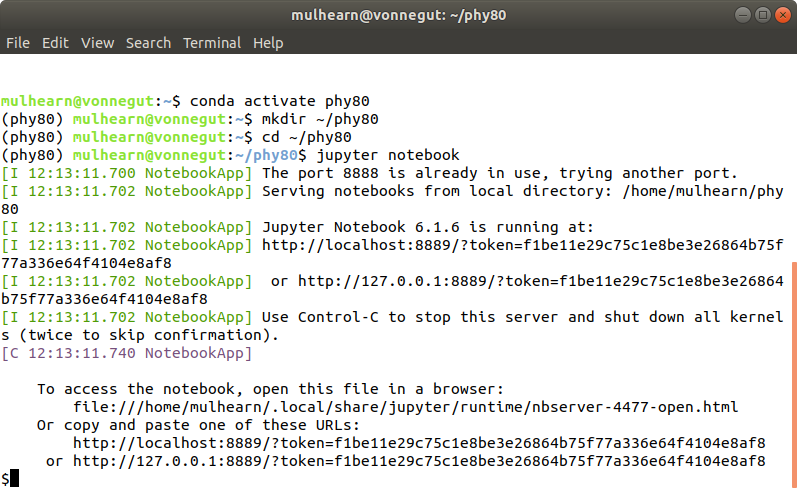
\includegraphics[width=0.65\textwidth]{figs/plotting/jupyter_startup.png} 
\caption{Example starting Jupyter Notebook from the Linux command line.  In Windows, you will need to open the Anaconda Prompt instead of a terminal.}
\label{fig:jupyterstartup}
\end{center}
\end{figure}

\begin{figure}[htbp]
\begin{center}
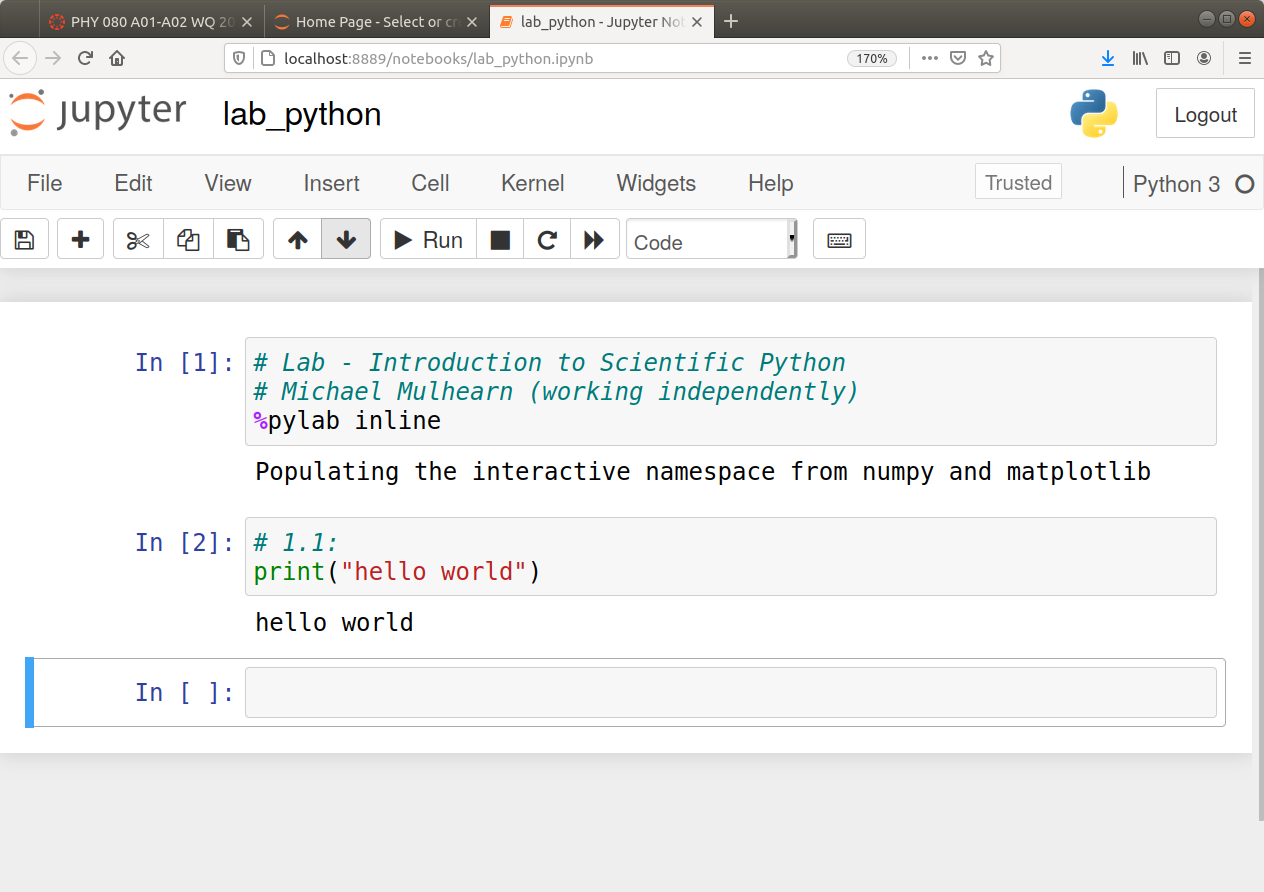
\includegraphics[width=0.65\textwidth]{figs/plotting/jupyter_window.png} 
\caption{The Hello World example Jupyter Notebook.}
\label{fig:jupyterwindow}
\end{center}
\end{figure}

\begin{figure}[htbp]
\begin{center}
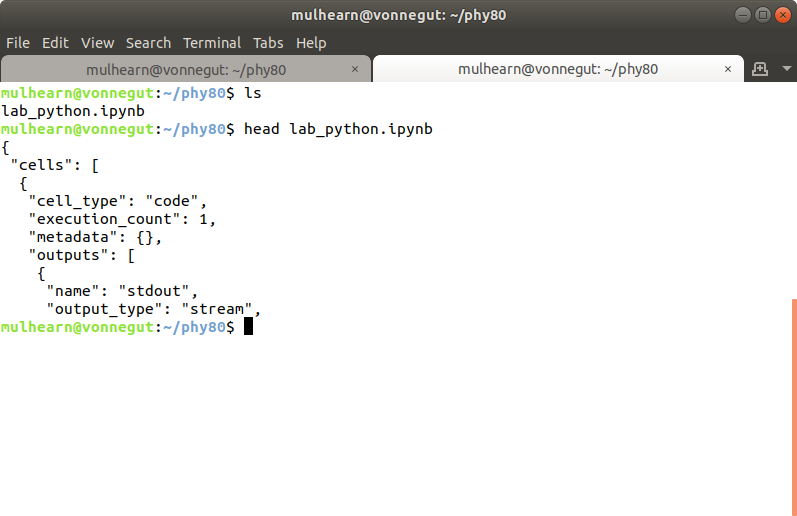
\includegraphics[width=0.65\textwidth]{figs/plotting/jupyter_saved.png} 
\caption{Example showing the saved Jupyter notebook.  Notice that notebook file (ipynb) is not human readable on its own: it requires the Jupyter software to render it in a human readable form.}
\label{fig:jupytersaved}
\end{center}
\end{figure}

After following the software installation instructions on the course
website, activate the Physics 80 environment with:
\begin{verbatim}
$ conda activate phy80
\end{verbatim}
Then, navigate to a working directory for this session, and start the notebook with:
\begin{verbatim}
$ jupyter notebook
\end{verbatim}
This should start the Jupyter Notebook server and open a client in your web browser.
An example starting a Jupyter Notebook from Linux is shown in Fig.~\ref{fig:jupyterstartup}.

You should create one Jupyter Notebook per lab assignment, by choosing
the New (Python 3) option in your client.  Change the name of your
notebook to something that clearly identifies the lab.  Start each lab
with comments (starting with ``\#'' symbol) indicating the title of
the lab, then your name followed by your lab partners.  See the first
cell of Fig.~\ref{fig:jupyterwindow} for an example.  This first cell
is also a good place to issue the ipython ``magic function'':
\begin{verbatim}
%pylab inline
\end{verbatim}
which will setup the notebook for inline plots and load the numpy and matplotlib libraries for you.

Each assignment will consist of a number of steps, clearly numbered like this one, you first step:

\begin{plot}
Print ``hello world'' using the python print command.
\end{plot}
\noindent
To keep your notebook clear, label cells (such as this one) with a
comment for the assignment step number, as in the second cell of
Fig.~\ref{fig:jupyterwindow}.  You only need to label one cell if
the assignment is fullfilled across several cells.

Jupyter Notebook checkpoints your work automatically.  You should be
able to see your notebook saved in the working directory where you
started, as in Fig.~\ref{fig:jupytersaved}.  Notice that while the
notebook file is ASCII text, it is not a human readable format.  The
Jupyter software is needed to render the notebook in a human readable
way.  To make your grader's life easier, you will be submitting PDF
versions of your notebook, once all of the tasks are completed and the
output is visible.  There are several ways to make a PDF file from
your notebook, but the most reliable is to use the ``Print Preview''
option to view the notebook as a PDF file within your browser, then
use the print feature of your browser to print the page as a PDF file.
Try this now, and make sure you can create a legible PDF file, but do
not submit it to the course site, as you still have more to do.
Always keep your python notebook file (ipynb) even after you submit
the assignment.  If you have problems, you can reproduce a PDF file
from the notebook file, but it is tedious to reproduce your notebook
from PDF.  If you have problems producing the PDF file, you can submit
the ``ipynb'' file as a temporary work-around, but work with your TA
to sort out the problem as quickly as possible.

\section{Submitting your assignment}

Before submitting, take some time to clean up your assignments to
remove anything superfluous and place the exercises in the correct
order.  You can also add comments as needed to make your work clear.
You can use the Cell $\to$ All Output $\to$ Clear and Cell $\to$ Run
All commands to make sure that all your output is up to date with the
cell source.

When you are satisfied with your work, print the PDF file as described
earlier and submit it to the course website.









